\documentclass[submit]{smj}
\usepackage{multirow}
\usepackage{subcaption}
\usepackage{adjustbox}

\def\E{\mathbb{E}}
\def\P{\mathbb{P}}
\def\bE{\mathbf{E}} 
\def\C{\mathcal{C}}
\def\by{\mathbf{y}}
\def\bY{\mathbf{Y}}
\def\bZ{\mathbf{Z}}
\def\bA{\mathbf{A}}
\def\bB{\mathbf{B}}
\def\bC{\mathbf{C}}
\def\bBb{\breve{\mathbf{B}}}
\def\1{\mathbf{1}}
\def\bbeta{\boldsymbol{\beta}}
\def\balpha{\boldsymbol{\alpha}}
\def\bgamma{\boldsymbol{\gamma}}
\def\bmu{\boldsymbol{\mu}}
\def\bX{\mathbf{X}}
\def\be{\boldsymbol{\e}}
\def\bSigma{\boldsymbol{\Sigma}}
\def\bGamma{\boldsymbol{\Gamma}}
\def\bV{\mathbf{V}}
\def\bI{\mathbf{I}}
\def\bJ{\mathbf{J}}
\def\b1{\mathbf{1}}
\def\bP{\mathbf{P}}
\def\bD{\mathbf{D}}
\def\sigmahat{\hat{\sigma}}
\def\sigmatilde{\tilde{\sigma}}
\def\Chat{\hat{\C}}
\def\Ctilde{\tilde{\C}}
\def\bV{\mathbf{V}}
\def\bVtilde{\tilde{\bV}}
\def\bSigmatilde{\tilde{\bSigma}}
\def\bSigmahat{\hat{\bSigma}}
\def\bbetatilde{\tilde{\bbeta}}
\def\vec{\textnormal{vec}}
\def\be{\mathbf{e}}
\def\bH{\mathbf{H}}
\def\bYtilde{\tilde{\bY}}
\def\diag{\textnormal{diag}}
\def\ddiag{\textnormal{ddiag}}
\def\bA{\mathbf{A}}
\def\bu{\mathbf{u}}
\def\bU{\mathbf{U}}
\def\bD{\mathbf{D}}
\def\bX{\mathbf{X}}
\def\bY{\mathbf{Y}}
\def\bM{\mathbf{M}}
\def\bw{\mathbf{w}}
\def\bff{\mathbf{f}}
\def\btheta{\boldsymbol{\theta}}
\def\bTheta{\boldsymbol{\Theta}}
\def\bx {\mathbf{x}}
\def\bz {\mathbf{z}}
\def\E{\mathbb{E}}
\def\bE{\mathbf{E}}
\def\cov{\textnormal{Cov}}
\def\C{\mathcal{C}}
\def\by{\mathbf{y}}
\def\bY{\mathbf{Y}}
\def\bB{\mathbf{B}}
\def\bBb{\breve{\mathbf{B}}}
\def\1{\mathbf{1}}
\def\bbeta{\boldsymbol{\beta}}
\def\balpha{\boldsymbol{\alpha}}
\def\bgamma{\boldsymbol{\gamma}}
\def\bX{\mathbf{X}}
\def\be{\boldsymbol{\e}}
\def\bSigma{\boldsymbol{\Sigma}}
\def\bGamma{\boldsymbol{\Gamma}}
\def\bV{\mathbf{V}}
\def\bI{\mathbf{I}}
\def\bJ{\mathbf{J}}
\def\b1{\mathbf{1}}
\def\bP{\mathbf{P}}
\def\bD{\mathbf{D}}
\def\sigmahat{\hat{\sigma}}
\def\sigmatilde{\tilde{\sigma}}
\def\Chat{\hat{\C}}
\def\Ctilde{\tilde{\C}}
\def\bV{\mathbf{V}}
\def\bVtilde{\tilde{\bV}}
\def\bSigmatilde{\tilde{\bSigma}}
\def\bSigmahat{\hat{\bSigma}}
\def\bbetatilde{\tilde{\bbeta}}
\def\vec{\textnormal{vec}}
\def\be{\mathbf{e}}
\def\bH{\mathbf{H}}
\def\bYtilde{\tilde{\bY}}
\def\diag{\textnormal{diag}}
\def\ddiag{\textnormal{ddiag}}
\def\bA{\mathbf{A}}
\def\bu{\mathbf{u}}
\def\bU{\mathbf{U}}
\def\var{\textnormal{var}}
\def\bV{\mathbf{\mathcal{V}}}
\def\bD{\mathbf{\mathcal{D}}}
\def\bR{\mathbf{\mathcal{R}}}
\def\bP{\mathbf{\mathcal{P}}}
\def\bxi{\boldsymbol{\xi}}
\def\bW{\mathbf{\mathcal{W}}}
\def\bpsi{\boldsymbol{\psi}}
\def\bPsi{\boldsymbol{\Psi}}
\def\bphi{\boldsymbol{\phi}}
\def\bPhi{\boldsymbol{\Phi}}
\def\bT{\mathbf{T}}
\def\bepsilon{\boldsymbol{\epsilon}}
\def\bLambda{\boldsymbol{\Lambda}}
\def\bOmega{\boldsymbol{\Omega}}
\def\bzeta{\boldsymbol{\zeta}}
\def\beeta{\boldsymbol{\eta}}
\def\btheta{\boldsymbol{\theta}}
\def\bC{\mathcal{C}}
\def\br{\mathbf{r}}

%%%%% PREAMBLE
%%%%% =============================================================================


%%% Place for putting personal \usepackage and \newcommand commands
%%% Note that some packages are loaded automatically
%%% with the smj class. 
%%% These include: graphicx, color, fancyvrb, amsmath, amssymb, calc, upquote (if available), natbib, url, hyperref.
%%%
%%% Please, specify all your personal definitions, newcommand etc. here
%%% and not inside the main body of the text.
%%% -------------------------------------------------------------------------------
%\usepackage{PACKAGE}
%\newcommand{MYCOMMAND}{...}

\Author{Ruonan Li\Affil{1}, 
       Luo Xiao\Affil{1}, 
       Ekaterina Smirnova\Affil{2},
       Erjia Cui\Affil{3},
       Andrew Leroux\Affil{4},
       %Jennifer A. Schrack \Affil{3},
        and Ciprian M. Crainiceanu\Affil{3}
        %and Emmanuel Lesaffre\Affil{4,}\Affil{5}
}
\AuthorRunning{R. Li \textrm{et al.}}


\Affiliations{

  %%% 1
\item Department of Statistics,
        North Carolina State University

  %%% 2
\item Department of Biostatistics, 
 Virginia Commonwealth University

  %%% 3
\item Department of Biostatistics, 
     Johns Hopkins Bloomberg School of Public Health
     
%%% 4
\item  Department of Biostatistics and Informatics, 
Colorado School of Public Health
}   %% end \Affiliations


%%% Postal, e-mail address, phone and fax of the corresponding author (not necessarily the first author).
%%% ------------------------------------------------------------------------------------------------------
%%% Use command \CorrAddress{} to provide a full postal address of the
%%% corresponding author in the form
%%% "Firstname Lastname, Department, University, Street 1, ZIP City, Country" 
%%% Use command \CorrEmail{} to provide an e-mail address of the corresponding author.
%%% Use command \CorrPhone{} to provide a phone number (including the country code!) of the corresponding author.
%%% Use command \CorrFax{} to provide a fax number (including the country code!) of the corresponding author.
\CorrAddress{Luo Xiao, 
             Department of Statistics, 
             North Carolina State University}
\CorrEmail{lxiao5@ncsu.edu}
\CorrPhone{(+1)\;919\;513\;4859}
\CorrFax{(+1)\;919\;513\;4859}


%%% Title and a short title (to be used as a running header) of the paper
%%% -------------------------------------------------------------------------------
\Title{Fixed-effects inference for longitudinal functional data}
\TitleRunning{Inference for longitudinal functional data}

%%% Abstract
%%% -------------------------------------------------------------------------------
\Abstract{
	We propose an inferential framework for fixed effects in longitudinal functional models and introduce tests for the correlation structures induced by the longitudinal sampling procedure. The framework provides a natural %and intuitive
	extension of standard longitudinal correlation models for scalar observations to functional observations. Using simulation studies, we compare fixed effects estimation under correctly and incorrectly specified correlation structures and provide explicit recommendations. We also apply the proposed methods to a longitudinal functional data set.
}


%%% Key words
%%% -------------------------------------------------------------------------------
\Keywords{
Accelerometry data; Covariance function; Hypothesis test;  Mixed effects model.
}


%%%%% MAIN BODY 
%%%%% =============================================================================
\begin{document}

%%% Title page
%%% -------------------------------------------------------------------------------
%%% Use command\maketitle to produce the title page.
\maketitle


%%% Main text
%%% ------------------------------------------
\section{Introduction}
Due to technological advancement, longitudinal functional data have become common in scientific studies \citep{Ramsay2005}. For example, objective physical activity measurements obtained from wearable accelerometers usually consists of multiple daily profiles measured at every minute of the day for hundreds or thousands of study participants at a number of visits. This type of data structure gives rise to longitudinal functional data \citep{Greven2010,Goldsmith2010}, which resembles traditional longitudinal data, but has a function instead of a scalar as the basic unit of observation. The average activity measured at multiple visits gives rise to standard longitudinal data, whereas  minute-by-minute activity profiles observed at multiple visits give rise to longitudinal functional data. 
Another example is brain imaging data, where through MRI scans, imaging data along brain tracts were collected for patients of multiple sclerosis and healthy controls at a number of visits. 
This new data structure requires specialized methodological tools to address scientific problems using the original structure of the data.

Longitudinal functional data often exhibit complex within- and between-function correlations. To accommodate such correlations, various functional mixed effects models have been proposed \citep{Di2009, Greven2010, Chen2012, Scheipl2015, Park2015,  Zhang2016, Chen2017,  Zhu2019, Lee2019}. These approaches, after data transformation or projections, allow inference on the fixed effects parameters using the linear mixed effects (LME) inferential machinery. Alternatively, bootstrap of study participants can be used to construct confidence bands and conduct hypothesis tests for fixed effect functions \citep{pmid22855258, Park2018, Zhu2019}. In spite of the growing interest in this area of research, modeling longitudinal functional data continues to be daunting. On the one hand, it is often difficult to specify within-function correlation structures that account for the continuity of the functional domain and are compatible with various sampling resolutions. On the other hand, the between-function correlations may be modeled flexibly using structured specifications that represent the known longitudinal sampling structure (e.g., nesting of functions within individuals). In this paper we consider a unified inferential model that explicitly separates the two types of correlations and propose to: (a) study the effects of misspecified longitudinal correlation structures on fixed effects inference for longitudinal functional data; (b) compare various longitudinal correlation structures proposed in the literature; and (c) propose testing methods for selecting the appropriate longitudinal correlation structure.

Our framework builds on the marginal decomposition model proposed by \cite{Park2015}, which focused on modeling the marginal covariance structure of longitudinal functional data, but did not consider fixed effects inference. We show that this approach can be used both for fixed effects inference and for the selection of appropriate longitudinal correlation models via hypothesis testing. For the latter, we extend the bootstrap-based approach for covariance testing proposed by \cite{Chen2019}. We will also show how this  framework can be used to compare models with different longitudinal correlation structures and evaluate the validity of marginal inferences under misspecified longitudinal correlation models.

In summary, the contributions of this paper are to, for longitudinal functional data: (a) generalize standard longitudinal correlation models; (b)  introduce testing for longitudinal correlation structures; and (c) study the effect of correctly and incorrectly specified correlation structures on the fixed effects inference.

The paper is organized as follows. In Section~\ref{sec:sec2},  we 
introduce the general functional mixed effects model and the specific longitudinal correlation structures for modeling longitudinal functional data. In Section~\ref{sec:test}, we address the problem of testing longitudinal correlation structure. Section~\ref{sec:simulations} assesses the properties of the statistical methods proposed using simulations.  Section~\ref{sec:application} applies our methods to real data. We conclude the paper with a discussion in Section~\ref{sec:conclusions}.

\section{Functional mixed effects models} \label{sec:sec2}

Let $\mathcal{T}\subset \mathbb{R}$ be a compact interval and the index $s\in \mathcal{T}$ be called the functional index. Let $y_{ij}(s)$ denote the observed response variable at $s$ for subject $i$,  $1\leq i\leq n$, at the $j$th,  $1\leq j\leq n_i$, visit that occurred at time $T_{ij}$. Denote by $\bx_{ij}  = [x_{ij1},\ldots, x_{ijp}]^{T}$ the vector of covariates for subject $i$ at visit $j$, and $\bx_i = [\bx_{i1}, \dots, \bx_{in_i}]^{T}$ the $n_i \times p$ matrix of covariates for subject $i$. Some of the covariates may depend on the visit number and some may not, but we use the index $j$ for all variables to simplify notation. For one data application on physical activity,  the covariates are age, body mass index (BMI) and sex, and thus $p=3$. Let $\by_{ij} = [y_{ij}(s_1),\ldots, y_{ij}(s_m)]^{T}$, where $\{s_1,\ldots, s_m\}$ is a fixed grid in $\mathcal{T}$. Let $\by_i = [\by^{T}_{i1},\ldots, \by^{T}_{in_i}]^{T}$ be the $mn_i$-dimensional column vector obtained by vectorizing all observations for subject $i$. 

We denote by $\mu_{ij}(\cdot)$ the conditional mean of the functional process $y_{ij}(\cdot)$ given the covariates $\bx_{ij}$ and assume that \begin{equation}\label{eq:mean}
\mu_{ij}(s) = \beta_0(s) + \sum_{r=1}^p x_{ijr} \beta_r(s)\;,
\end{equation}
where $\beta_r(\cdot)$ are smooth, unknown functions of $s$. Using the approach in \cite{Park2015}, we decompose the functional residuals, $y_{ij}(s) - \mu_{ij}(s)=W_{ij}(s) + \epsilon_{ij}(s)$, where
\begin{equation*}
W_{ij}(s) = \sum_{k\geq 1} \xi_{ijk} \phi_k(s)\;, 
\end{equation*}
and $\epsilon_{ij}(s)$ is white noise with zero mean and variance $\sigma_{\epsilon}^2$. The functions $\{\phi_1(\cdot), \phi_2(\cdot),\ldots\}$ form an orthonormal basis and $\xi_{ijk}$ are associated random  coefficients. We assume that $\xi_{ijk}$ are normally distributed with zero mean and covariance $G_k(T_{ij_1}, T_{ij_2}) = \text{Cov}\{\xi_{ij_1k},\xi_{ij_2k}|T_{ij_1}, T_{ij_2}\}$
and are uncorrelated over $i$ and $k$. Then the covariance of the process is a four-dimensional operator with the following structure $$\bC(s_1, T_{ij_1}, s_2, T_{ij_2}) = \text{Cov}\big\{W_{ij_1}(s_1), W_{ij_2}(s_2)|T_{ij_1}, T_{ij_2}\big\} = \sum_{k\geq 1} G_k(T_{ij_1},T_{ij_2}) \phi_k(s_1)\phi_k(s_2).$$
We also assume that the sampling visits $T_{ij}$ are independent over $i$ and $j$ and have a smooth probability density function, $g(\cdot)$.  Then the basis functions $\phi_k(\cdot)$ are eigenfunctions of the  marginal covariance operator 
$$\bC_m(s_1, s_2) = \int \bC(s_1,T, s_2,T) g(T)\mathrm{d}T = \sum_{k\geq 1}\lambda_k \phi_k(s_1)\phi_k(s_2),$$
where $\lambda_k = \int G_k(T,T)g(T)\mathrm{d}T$ are eigenvalues and are assumed to be ordered decreasingly, i.e.,  $\lambda_1\geq \lambda_2\geq\ldots\geq 0$, and the random coefficients $\xi_{ijk}$ satisfy $\xi_{ijk} = \int W_{ijk}(s)\phi_k(s)\mathrm{d}s$.


Standard longitudinal models use working covariance often assume either independence, exchangeability, or leave them unspecified. A natural generalization of these assumptions to longitudinal functional data is via the specification of the working covariance, $G_k(\cdot,\cdot)$, for every eigenfunction, $\phi_k(\cdot)$, indexed by $k$. We propose to model the within-function covariance nonparametrically and the between-function covariance using approaches inspired by  standard and functional longitudinal data analysis. The rationale is that the functions are often densely observed and exhibit complex correlation structure, for which a nonparametric approach would provide the needed flexibility, while the longitudinal sampling visits are often sparse, for which a simpler correlation structure might be sufficient and also easy to interpret. 


\subsection{Longitudinal working covariances}
We consider three common correlation models including two parametric correlation structures, but methods can easily be extended to other parametric correlation structures. 

The first is the working independence model, where $W_{ij}(\cdot)$ are assumed to be independent and identically distributed for all $i$ and $j$.
Under this framework the random scores $\xi_{ijk} = \zeta_{ijk}$, where $\zeta_{ijk}$ are uncorrelated across $i$ and $j$ for each $k$ and $\text{Var}(\zeta_{ijk}) = \sigma_{e, k}^2$. Then, we have $G_k(T_{ij_1},T_{ij_2}) = \sigma_{e, k}^2 1_{\{j_1= j_2\}}$.


The second is the exchangeable correlation model, that is
$\xi_{ijk} = \xi_{ik} + \zeta_{ijk}$, where $\xi_{ik}$ is uncorrelated with all $\zeta_{ijk}$
and $\zeta_{ijk}$ are mutually uncorrelated for all $i$, $k$ and $j$. Denote $\sigma_{0, k}^2 =  \text{Var}(\xi_{ik})$ and $\sigma_{e, k}^2 =  \text{Var}(\zeta_{ijk})$, and then
$G_k(T_{ij_1},T_{ij_2}) = \sigma_{0, k}^2+\sigma_{e, k}^21_{\{j_1=j_2\}}$. The exchangeable model for longitudinal functional data is a particular case of the multilevel functional principal component model of \citet{Di2009}. Indeed, we may write $W_{ij}(s)$ as $U_i(s) + V_{ij}(s)$ with $U_i(s) = \sum_{k\geq 1} \xi_{ik}\phi_k(s)$ and $V_{ij}(s) = \sum_{k \geq 1} \zeta_{ijk} \phi_k(s)$. 


The third is the unspecified  smooth correlation model, where $G_k(\cdot,\cdot)$ is modeled nonparametrically. In this case $\xi_{ijk} = \xi_{ik}(T_{ij}) + \zeta_{ijk}$, where $\xi_{ik}(T_{ij})$ is a zero-mean smooth process with covariance function $\text{Cov}\big\{\xi_{ik}(T_{ij_1}), \xi_{ik}(T_{ij_2})\big\} = G_{k0}(T_{ij_1}, T_{ij_2})$, and $\zeta_{ijk}$ are zero mean random errors with $\text{Var}(\zeta_{ijk}) = \sigma_{e,k}^2$. In particular, $\zeta_{ijk}$ are mutually uncorrelated for all $i, j$ and $k$. The induced covariance function is $G_k(T_{ij_1},T_{ij_2})= G_{k0}(T_{ij_1}, T_{ij_2}) + \sigma_{e, k}^2 1_{\{j_1=j_2\}}$. We further decompose the covariance function $G_{k0}(T_{ij_1}, T_{ij_2})$ as $G_{k0}(T_{ij_1}, T_{ij_2}) = \sum_{\ell=1}^{\infty} \lambda_{k\ell} \psi_{k\ell}(T_{ij_1})\psi_{k\ell}(T_{ij_2})$, where $\lambda_{k1}\geq \lambda_{k2}\geq\cdots\geq 0$ and $\psi_{k\ell}(\cdot)$ are orthonormal eigenfunctions that satisfy $\int_{T} \psi_{k\ell_1}(T)\psi_{k\ell_2}(T)\mathrm{d}T = 1_{\{\ell_1\neq \ell_2\}}$. It follows that $\xi_{ijk}$ can be written as $\sum_{\ell=1}^{\infty}\eta_{ik\ell}\psi_{k\ell}(T_{ij}) + \zeta_{ijk}$,
where $\eta_{ik\ell}$ are uncorrelated random scores with zero mean and variance $\lambda_{k\ell}$.


The unspecified smooth covariance model contains the independent and exchangeable models as special cases. Indeed, the working independence model corresponds to $G_{k0}(T_{ij_1},T_{ij_2}) = 0$ while the exchangeable correlation model corresponds to  $G_{k0}(T_{ij_1},T_{ij_2}) = \sigma_{0, k}^2$. Thus, for model estimation below, we will focus on the unspecified covariance model as the other cases can be treated as simpler cases. 


\subsection{Model estimation} \label{sec:Modelestimation}
We first consider estimation of $\mu_{ij}(\cdot)$ using B-spline expansion of the coefficient functions $\beta_r(\cdot)$. Specifically, let $\bB(s) = [B_1(s),\ldots, B_c(s)]^{T}\in \mathbb{R}^c$ be a collection of B-spline basis functions in the unit interval with $c$ being the number of basis functions. Then $\beta_r(s) = \sum_{d=1}^c \alpha_{rd} B_{d}(s)$, where $\balpha_r = [\alpha_{r1},\ldots, \alpha_{rc}]^{T}$ is the unknown coefficient vector. 
We use c and a relatively large number of equally spaced knots, i.e., a large $c$, so that the approximation bias is negligible. Let $\bB =[\bB(s_1),\ldots, \bB(s_m)]^T\in \mathbb{R}^{m\times c}$, then
$\bmu_{ij} = [\mu_{ij}(s_1),\ldots, \mu_{ij}(s_m)]^T = \bB\balpha_0 + \sum_{r=1}^p x_{ijr}\bB\balpha_r$. Denote
$\bX_{ij} = [\bB, x_{ij1}\bB,\ldots, x_{ijp}\bB]\in \mathbb{R}^{m\times ((p+1)c)}$, 
$\balpha= [\balpha^T_0,\ldots,\balpha^T_p]^T\in\mathbb{R}^{(p+1)c}$. Then, we have
$\bmu_{ij} = \bX_{ij}\balpha$.
Let $\bX_i = [\bX^T_{i1},\ldots,\bX^T_{in_i}]^T\in \mathbb{R}^{(mn_i)\times ((p+1)c)}$
and $\bmu_i = [\bmu^T_{i1},\ldots, \bmu^T_{in_i}]^T\in \mathbb{R}^{mn_i}$. Then, we have $\bmu_i = \bX_i \balpha$. 



Now we consider  $W_{ij}(s) = \sum_{k\geq 1} \xi_{ijk}\phi_k(s)\;,$
where for each $k\geq 1$, $\xi_{ijk} = \sum_{\ell\geq 1} \eta_{ik\ell} \psi_{k\ell}(T_{ij}) + \zeta_{ijk}\;.$ As both terms involve infinite sums, we propose to use a number of eigenfunctions $\phi_k(\cdot)$ that explains at least a given percentage of the variance explained (PVE) in the marginal covariance function, $\C_m$. Denote the selected number of $\phi_k(\cdot)$ by $K$. Next we determine the approximation of $\xi_{ijk}$ for all $1\leq k\leq K$ simultaneously by ranking $\lambda_{k\ell}$, the variances of scores $\eta_{ik\ell}$.
We retain the $\lambda_{k\ell}$ that are larger than $\lambda^{\ast}$, where $\lambda^{\ast}$ is the largest value that satisfies 
\begin{equation*}
	\frac{\sum_{k=1}^K\sigma^2_{e,k} + \sum_{k\geq 1}\sum_{\ell\geq 1} \lambda_{k\ell} 1_{\{\lambda_{k\ell}\geq \lambda^{\ast}\}} }{\sum_{k=1}^K\sigma^2_{e,k} + \sum_{k\geq 1}\sum_{\ell\geq 1}\lambda_{k\ell} }  > \text{PVE}\;.
\end{equation*}
This will discard $\eta_{ik\ell}$ with small variances and, according to our simulation studies, is a useful procedure for stabilizing the estimation. Let $L_k$ be the number of eigenfunctions selected for $\xi_{ijk}$. Then approximately,
\begin{equation*}
W_{ij}(s) = \sum_{1\leq k\leq K}\left\{ \sum_{1\leq \ell\leq L_k} \eta_{ik\ell} \psi_{k\ell}(T_{ij}) + \zeta_{ijk} \right\}\phi_k(s)\;.
\end{equation*}
Let $\boldsymbol{W}_{ij} = [W_{ij}(s_1),\ldots, W_{ij}(s_m)]^{T}\in\mathbb{R}^{m}$, $\bphi_{k} = [\phi_{k}(s_1),\ldots, \phi_{k}(s_m)]^{T}\in\mathbb{R}^{m}$,
$\bPsi_{ijk} = [\psi_{k1}(T_{ij}),\ldots, \psi_{kL_k}(T_{ij})]^{T}\in \mathbb{R}^{L_k}$, and 
$\beeta_{ik} = [\eta_{ik1},\ldots, \eta_{ikL_k}]^{T}\in\mathbb{R}^{L_k}$. Then
\begin{equation*}
\boldsymbol{W}_{ij} = \sum_{1\leq k\leq K}\left( \bPsi_{ijk}^{T}\beeta_{ik}+ 
\zeta_{ijk}\right)\bphi_k\;.
\end{equation*}
Let $\bPsi_{ij} = \text{blockdiag}(\bPsi_{ij1}^{T},\ldots, \bPsi_{ijK}^{T})\in \mathbb{R}^{K\times L}$, where $L = \sum_{1\leq k\leq K} L_k$, and $\beeta_i = [\beeta_{i1}^{T},\ldots, \beeta_{iK}^{T}]^{T}\in\mathbb{R}^{L}$. Note that $\beeta_{ik}$ has a diagonal covariance matrix $\bLambda_k = \text{diag}(\lambda_{k1},\ldots, \lambda_{kL_k})$ and $\beeta_i$ has a diagonal covariance matrix $\bLambda = \text{blockdiag}(\bLambda_1,\ldots, \bLambda_K)$. Let $\bPhi = [\bphi_1,\ldots, \bphi_K]\in \mathbb{R}^{m\times K}$ and $\bzeta_{ij} = [\zeta_{ij1},\ldots, \zeta_{ijK}]^{T} \in \mathbb{R}^{K}$. Then
\begin{equation*}
\boldsymbol{W}_{ij} = \bPhi\left(\bPsi_{ij}\beeta_{i} + \bzeta_{ij}\right)\;.
\end{equation*}
Let $\boldsymbol{W}_i = [\boldsymbol{W}_{i1}^{T},\ldots, \boldsymbol{W}_{in_i}^{T}]^{T}\in
\mathbb{R}^{mn_i}$, $\bPsi_i =[\bPsi^{T}_{i1},\ldots, \bPsi^{T}_{in_i}]^{T} \in \mathbb{R}^{(Kn_i) \times L }$, and $\bzeta_i = [\bzeta^{T}_{i1},\ldots, \bzeta^{T}_{n_ii}]^{T} \in \mathbb{R}^{Kn_i}$. Then
\begin{equation*}
\boldsymbol{W}_i = (\mathbf{I}_{n_i}\otimes \bPhi)\left(
\bPsi_i\beeta_i  + \bzeta_i\right)\;.
\end{equation*}
It is easy to show that $\bzeta_{ij}$ has a diagonal covariance matrix $\bSigma = \text{diag}(\sigma_{e,1}^2,\ldots, \sigma_{e,K}^2)$ and that $\bzeta_i$ has a diagonal covariance matrix $\mathbf{I}_{n_i}\otimes\bSigma$. For the random error term $\epsilon_{ij}(s)$, let $\bepsilon_{ij} = [\epsilon_{ij}(s_1),\ldots, \epsilon_{ij}(s_m)]^{T}\in\mathbb{R}^m$ and $\bepsilon_{i} = [\bepsilon^{T}_{i1},\ldots, \bepsilon^{T}_{in_i}]^{T} \in \mathbb{R}^{mn_i}$. 

Finally, we obtain the mixed model representation
\begin{equation} \label{eq:mixed}
\begin{split}
\by_i &= \bX_i \balpha +  (\mathbf{I}_{n_i}\otimes \bPhi)\left(
\bPsi_i\beeta_i  + \bzeta_i\right) + \bepsilon_i,\\
\begin{pmatrix}\beeta_i\\ \bzeta_i \\\bepsilon_i\end{pmatrix}&\sim \mathcal{N}\left[
\begin{pmatrix} \mathbf{0}_{L}\\\mathbf{0}_{Kn_i}\\\mathbf{0}_{mn_i}\end{pmatrix},
\begin{pmatrix} \bLambda&0&0\\0&\mathbf{I}_{n_i}\otimes\bSigma&0\\ 0&0&\sigma_{\epsilon}^2\bI_{mn_i}\end{pmatrix}
\right]\;,
\end{split}
\end{equation}
where $[\beeta^{T}_i, \bzeta^{T}_i,\bepsilon^{T}_i]^{T}$ are independent across subjects. Therefore, given the eigenfunctions $\bPsi_i$ and $\bPhi$,  the fixed effects $\balpha$ and variance components $\lambda_{k\ell}$, $\sigma_{e,k}^2$, and $\sigma_{\epsilon}^2$ can be estimated using standard mixed effects software. To avoid overfitting, we impose a quadratic penalty on each $\balpha_r$. Let $\bP$ be a second order difference penalty matrix \citep{Eilers1996}. To be specific we use the penalty $\sum_{r=0}^p \tau_r \balpha^{T}_r\bP\balpha_r$, where $\tau_r$ is the smoothing parameter for the $r$th function $\beta_r(\cdot)$. The model can be fitted using the {\it gam} function \citep{Wood2016} in the R package {\it mgcv} \citep{mgcv2019} and we use generalized cross validation to select the smoothing parameters.


\subsection{Longitudinal  covariance estimation} 

We will use an iterative procedure between estimating the mean and covariance structure, respectively. First, assume  that $\balpha$ is estimated, and thus $\beta_r(\cdot)$s, are known. Then the residuals $r_{ij}(s) = y_{ij}(s) - \mu_{ij}(s)$ can be calculated. 
An initial estimate of $\balpha$ can be obtained, for example, by fitting
model~\eqref{eq:mixed} without including the term $(\mathbf{I}_{n_i}\otimes \bPhi)\left(
\bPsi_i\beeta_i  + \bzeta_i\right)$. This is equivalent to assume that all observations $y_{ij}(s)$ are mutually independent.

Once the residuals are estimated, the eigenfunctions $\phi_k(\cdot)$ can be estimated by using the fast {\it face} algorithm \citep{Xiao2016} of the sandwich smoother \citep{Xiao2013} on the set of pooled residuals, $r_{ij}(s)$. Specifically, let $\boldsymbol{R}_{ij} = [r_{ij}(s_1),\ldots, r_{ij}(s_m)]^{T} \in \mathbb{R}^m$, 
$\boldsymbol{R}_i = [\boldsymbol{R}_{i1},\ldots, \boldsymbol{R}_{in_i}] \in \mathbb{R}^{m\times n_i}$ and $\boldsymbol{R} = [\boldsymbol{R}_1,\ldots, \boldsymbol{R}_n]\in \mathbb{R}^{m\times N}$, where $N = \sum_{i=1}^n n_i$. Then we apply the {\it face} algorithm to $N^{-1} \boldsymbol{R}\boldsymbol{R}^{T}$.

Given $\phi_k(\cdot)$, we  calculate $\int r_{ij}(s)\phi_k(s)\mathrm{d}s$ as the prediction for $\xi_{ijk}$.
For the working independence model,
$\lambda_k$ can be estimated along with $\phi_k(\cdot)$ directly.
For the exchangeable model, we have $\xi_{ijk} = \xi_{ik} + \zeta_{ijk}$ and a one-way nested ANOVA model can be used to estimate $\sigma_{0,k}^2$ and $\sigma_{e,k}^2$. Finally, when $G_k(\cdot,\cdot)$ is unspecified, we use the fast covariance estimation method for sparse functional data \citep{Xiao2018}
to $\xi_{ijk}$ to obtain estimates of $G_{k0}(\cdot,\cdot)$ and $\sigma_{e,k}^2$ for each $k$.


\section{Tests of longitudinal covariances} \label{sec:test}
We  use the goodness of fit test in \citet{Chen2019} to test the  structure of the  covariance $G_{k0}(\cdot,\cdot)$ in the following scenarios: (1) test the independent model against the unspecified covariance model; and (2) test the exchangeable model against the unspecified covariance model. Tests with specified parametric alternatives in a similar setting have been considered in \citet{Park2015}. We will consider two types of tests: test of an individual covariance or joint test of multiple covariances. 
To illustrate the idea, consider the case when the null hypothesis assumes  independence. For the individual test, we may test $H_{0k}: G_{k0}(\cdot, \cdot) = 0$ against $H_{1k}: G_{k0}(\cdot,\cdot)$ is unspecified for each $k$.  For the joint test, we may test $H_0: G_{k0}(\cdot,\cdot) = 0$ for all $k\geq 1$ against $H_1: G_{k0}(\cdot,\cdot)$ is unspecified for at least  one $k\geq 1$. The null model for the joint test corresponds to the assumption that the longitudinal functions $W_{ij}(\cdot)$ are uncorrelated across visits, $j$, within study participants.

\subsection{Individual longitudinal covariance test}

The hypothesis test can be written as 
\begin{equation}
\label{eq:hypotest}
H_{0k}: G_{k0}(T,T^{\prime})=\widetilde{G}_{k0}(T,T^{\prime}) \quad\text{versus}\quad H_{1k}: G_{k0}(T,T^{\prime}) \neq \widetilde{G}_{k0}(T,T^{\prime})\;,
\end{equation}
where $\widetilde{G}_{k0}(T,T^{\prime})$ is a parametric covariance function with a finite number of unknown parameters. For example, to test the null hypothesis of an exchangeable covariance model, we have $G_{k}(T_{ij_1},T_{ij_2}) = \widetilde{G}_{k0}(T_{ij_1},T_{ij_2}) + 1_{\{j_1=j_2\}}\sigma^2_{e,k}$, where $\widetilde{G}_{k0}(T_{ij_1},T_{ij_2}) = \sigma^2_{0,k}$.
For testing the null hypothesis of working independence, everything stays the same, except that $\widetilde{G}_{k0}(T_{ij_1},T_{ij_2}) = 0$.

We now briefly describe the test proposed in \citet{Chen2019}. Suppose that the null covariance is $G_0$ and the alternative is $G_A$.
First, we estimate the unknown parameters under the null hypothesis and denote the resulting estimate by $\widehat{G}_0$.
Under the alternative hypothesis, we estimate $G_A$ nonparametrically using, for example, smoothing based on  tensor product of B-splines. If the estimator under the alternative hypothesis is $\widehat{G}_A$ then the test statistic is the Hilbert-Schmidt norm distance
\begin{equation*}
T_n = \left\|\widehat{G}_A - \mathcal{K} \widehat{G}_0\right\|_{HS}\;,
\end{equation*}
where $\left\|f\right\|_{HS}=\sqrt{\iint f(T,T^{\prime})^2\mathrm{d}T \mathrm{d}T^{\prime}}$ and $\mathcal{K}\widehat{G}_0$ is the smoothed null covariance estimate using again tensor-product of B-splines. The rationale for  smoothing $\widehat{G}_0$ is to remove the potential bias induced by smoothing procedure used for obtaining $\widehat{G}_A$.  Larger values of the test statistic, $T_n$, will provide evidence against the null hypothesis.  The null distribution of $T_n$ is obtained via wild bootstrap \citep{Wu1986}, i.e., the estimated error variance under the alternative hypothesis is used to generate bootstrap samples.


\subsection{Joint test of multiple longitudinal covariances}

To explore the overall structure of longitudinal covariances for modeling  longitudinal functional data, we propose a joint test of $G_{k0}(\cdot,\cdot)$ for all $1 \leq k \leq K$. The approach we propose is straightforward: conduct individual covariance tests and use a Bonferroni correction to control the family-wise error rate.


\section{Simulation studies} \label{sec:simulations} 

We use simulations to compare the performance of inferential approaches for the longitudinal functional models using independent, exchangeable, and unspecified covariance assumptions. We will focus on estimation and inference for fixed effects as well as size and power of the covariance tests introduced in Section~\ref{sec:test}. The longitudinal functional models are compared with the standard functional data method implemented  in the {\it pffr} function \citep{Ivanescu2015, Scheipl2015, Scheipl2016} of the R package {\it refund} \citep{refund2018}. This approach was designed for functional data without residual correlation and will be referred to as the naive method, in the sense that the method is naive to the longitudinal correlation assumptions. The methods implemented in the {\it pffr} function work very well in practice when residuals are not correlated. We also compare methods with the  bootstrap method  \citep{ Park2018} to obtain the confidence bands for the coefficient functions. The point estimators for the bootstrap approach are obtained using the {\it pffr} function.


\subsection{Simulation settings}\label{subsec:sim_scenarios}

Data are generated from the model   $y_{ij}(s) = \mu_{ij}(s) + W_{ij}(s) + \epsilon_{ij}(s),\, s\in [0,1]$.  The functional mean is 
$\mu_{ij}(s)=\beta_0(s) + x_{i1}\beta_1(s)+x_{ij2}\beta_2(s),$ where the number of covariates is $p=2$, $x_{i1} \overset{iid}{\sim} N(0,1)$, and $x_{ij2}=aT_{ij}+ e_{ij}$, where $e_{ij}\sim N(\rho e_{i(j-1)}, 1)$ with $e_{i0} = 0$. We let $a = 1$ and $\rho = 0.7$.  The coefficient functions are  $\beta_0(s) = 1 + \sqrt{3}\cos(3\pi s)$, $\beta_1(s) = 2 + \cos(2\pi s)$ and   $\beta_2(s) = 2 + \sin(\pi s)$. The number of visits per subject, $m_i$, will be specified later while the visit times, $T_{ij}$, are generated uniformly from the unit interval and then ordered.   Using the orthonormal functions $\phi_1(s) = 1$ and $\phi_2(s) = \sqrt{2}\sin(2\pi s)$, $W_{ij}(\cdot)$ is generated from one of the three models below:
\begin{enumerate}
	\item Independent covariance: $W_{ij}(s) = \sum_{k=1}^2 \zeta_{ijk} \phi_k(s)$\;.
	\item Exchangeable covariance: $W_{ij}(s) = \sum_{k=1}^2 (\xi_{ik} + \zeta_{ijk}) \phi_k(s)$\;.
	\item Unspecified covariance: $W_{ij}(s) = \sum_{k=1}^2 \left\{
	\sum_{\ell=1}^2 \eta_{ik\ell} \psi_{k\ell}(T_{ij}) + \zeta_{ijk} \right\}\phi_k(s)$\;.
\end{enumerate}
For the independent covariance, $\zeta_{ij1} \overset{iid}{\sim}  N(0, 4.5)$
and $\zeta_{ij2} \overset{iid}{\sim} N(0, 3)$.
For the exchangeable covariance, $\xi_{i1} \overset{iid}{\sim}  N(0,3)$,
$\xi_{i2} \overset{iid}{\sim} N(0, 2)$, $\zeta_{ij1} \overset{iid}{\sim}  N(0,1.5)$
and $\zeta_{ij2} \overset{iid}{\sim}  N(0, 1)$. For the unspecified covariance, $\psi_{11}(T) = \sqrt{2}\cos(2\pi T)$, $\psi_{12}(T) = \sqrt{2}\sin(2\pi T)$, $\psi_{21}(T) = \sqrt{2}\cos(4\pi T)$, and  $\psi_{22}(T) = \sqrt{2}\sin(4\pi T)$. We generate the random terms as $ \eta_{i11}  \overset{iid}{\sim} N(0,2)$, $\eta_{i12}  \overset{iid}{\sim} N(0,1.5)$, $\eta_{i21}  \overset{iid}{\sim} N(0, 1.5)$, $\eta_{i22}  \overset{iid}{\sim} N(0,1)$, $\zeta_{ij1} \overset{iid}{\sim}  N(0, 1)$ and $\zeta_{ij2} \overset{iid}{\sim} N(0, 0.5)$. The functional arguments $\{s_1, \dots, s_m \}$ form a grid of $101$ equidistant points in the unit interval.


The mutually independent random errors $\epsilon_{ij}(s)$
are generated  from $N(0, \sigma_{\epsilon}^2)$. The value of $\sigma_{\epsilon}^2$ is $1.5$, which is determined by 
a signal to noise ratio (SNR) with a value of $5$. For the independent and exchangeable covariances, 
we defined SNR in the functional data as ${\sum_{k\geq 1}(\sigma^2_{0,k} +  \sigma^2_{e,k})}/{\sigma_{\epsilon}^2}$; for the unspecified covariance, we defined SNR as ${\sum_{k\geq 1} ( \sum_{\ell\geq 1} \lambda_{k\ell} +  \sigma^2_{e,k})}/{ \sigma_{\epsilon}^2}$.

For simulations, we used a factorial design with three factors: (a) the number of subjects is either $100$ or $200$; (b) the number of visits $m_i$ are generated from either $\text{Unif}[3,\ldots, 6]$ or $\text{Unif}[8,\ldots, 12]$; and (c) the covariance model is either independent, exchangeable or unspecified. There are $12$ model conditions and for each condition we simulate $500$ datasets. 

For tests of longitudinal covariances,
data are generated similarly. However, under the alternative we add terms  to ensure that the null model is misspecified. Specifically, we consider
\begin{enumerate}
	\item Deviation from independent covariance: $\xi_{ijk}\rightarrow \xi_{ijk} + \Delta z_{ik}(T_{ij})$\;.
	\item Deviation from exchangeable covariance: $\xi_{ik} + \zeta_{ijk}\rightarrow \xi_{ik} + \zeta_{ijk}+ \Delta z_{ik}(T_{ij})$\;.
\end{enumerate}
The scalar $\Delta$ controls the magnitude of the deviation from the null model. The scores $\xi_{ik}$ and $\zeta_{ijk}$ are independent from the non-linear random function $z_{ik}(\cdot)$, where $z_{ik}(T) = \sum_{\ell=1}^2\eta_{ik\ell}\psi_{k\ell}(T)$. The terms $\eta_{ik\ell}$ and $\psi_{k\ell}(T)$ are specified as before.



\subsection{Model estimation and evaluation criteria}
The initial mean estimation is conducted using the {\it pffr} function using $10$ cubic B-splines bases and the second order difference penalty. The  marginal eigenfunctions $\phi_k(s)$ are estimated by fitting the  functional residuals  via the  {\it fpca.face} function \citep{Xiao2016} in the R package {\it refund} with $20$ knots. The unspecified covariance model components $\psi_{k\ell}(T)$ and $\xi_{ik\ell}$ are estimated using  the {\it face.sparse} function in the R package {\it face} with $15$ knots. The truncation parameters $K$ and $L_k$ (for the unspecified covariance model) are all determined using the pre-specified level percentage of variance explained (PVE) with a value of $0.95$. The final mixed model is fitted using {\it bam} function \citep{Wood2015} in the R package {\it mgcv} \citep{mgcv2019}.

The estimation accuracy for functional parameters is assessed using the mean integrated squared errors (MISE) and the properties of the pointwise confidence intervals. Specifically, for a function $\beta$ with estimate $\hat \beta$, $\text{MISE}(\hat \beta) = \frac{1}{N_{sim}}\sum_{i_{sim} =1}^{N_{sim}} \int \{\hat\beta^{i_{sim}}(s) - \beta(s)\}^2ds $. 
For the pointwise confidence intervals, we report the integrated actual pointwise coverage (IAC) and integrated actual width (IAW), where IAC is defined as $ \frac{1}{N_{sim}} \sum_{i_{sim} =1}^{N_{sim}} \int I\{\hat\beta^{i_{sim}}(s) \in CI_p(s)\}ds$ and $CI_p(s)$ is the pointwise approximate confidence interval for the functional parameter $\beta(s)$. For example, an approximate $95\%$ pointwise confidence interval $CI_p(s_0)$ for $\beta_1(s_0)$ can be constructed as $\beta_1(s_0) \pm 1.96\times\hat{\text{SD}}\{\hat \beta_1(s_0)\}$. The length of the confidence interval at $s_0$ is $3.92\times\hat{\text{SD}}\{\hat \beta_1(s_0)\}$ and $\text{IAW} = \frac{1}{N_{sim}}\sum_{i_{sim} =1}^{N_{sim}} \int 3.92\times\hat{\text{SD}}\{\hat\beta^{i_{sim}}(s)\}ds$. 


\subsection{Simulation results for estimation}\label{subsec:sim_results}

Tables~\ref{tab:linear2}, \ref{tab:linear4} and \ref{tab:linear6} display the results for estimating the coefficient functions when the data generating mechanism uses independent, exchangeable, or unspecified covariances, respectively. We first focus on the point estimation, which is partially captured by the MISE in the three tables. Results indicate that as the number of subjects and  visits increase, MISEs decrease for all methods; see the columns labeled $\sqrt{\rm MISE}$ in Tables~\ref{tab:linear2}, \ref{tab:linear4} and \ref{tab:linear6}. Moreover, the MISE obtains the smallest value when the correlation is correctly specified. In particular, the reduction in MISE is substantial for data with exchangeable and unspecified covariance structures when the correct model is used compared to one that does not account for correlation. For example, in Table~\ref{tab:linear4} which corresponds to data simulated from an exchangeable correlation structure, for $n=200$ and $m_i\sim {\rm Unif}[8,12]$, the $\sqrt{\rm MISE}$ was $0.12$ for $\beta_2(s)$ for the method which accounted for exchangeable correlation, while it was $0.28$ for the Park et al. method which did not. Finally, the unspecified correlation model consistently provides good estimators, with the corresponding MISE comparable to that obtained from the correctly specified model.

For confidence bands, all  methods outperform the naive method in terms of coverage. The confidence bands from the naive method are on average too narrow and are far below the nominal coverage level. The correctly-specified and the unspecified covariance models provide confidence bands that are close to the nominal, though,  slightly conservative sometimes. The bootstrap method  provides confidence bands that close to the nominal, though they require more computational times and have  higher average width for estimating slope functions and lower average width for estimating intercept functions. When models are misspecified (e.g., exchangeable model for unspecified covariance data), the average coverage of the confidence bands tends to be close to the nominal, but at the expense of much wider confidence bands.


In terms of running time, the bootstrap method is the slowest and the naive method is the fastest. Computational time increases with more complex longitudinal correlation structures. However, when the dataset has a large number of subjects and a large number of visits per subject ($n=200$ and $m_i\sim \text{Unif}[8,12])$, the computation time for fitting the proposed methods can be comparable to that of the bootstrap. 

In summary, the unspecified covariance models perform well in terms of inference for the fixed effects in a variety of scenarios. However, in practice one may still want to know whether a simpler correlation structure is reasonable for the data, as the correct model slightly outperforms the unspecified covariance model. In the next section, we provide results for testing the longitudinal covariance.

\begin{table}
	\centering
	\caption{$\sqrt{\text{MISE}}$,  IAC for $95\%$ pointwise confidence interval and IAW for estimating $\beta_0(s)$, $\beta_1(s)$ and $\beta_2(s)$ based on independent covariance data using five methods across $500$ simulations.}
	\label{tab:linear2}
	\begin{adjustbox}{width=\textwidth}
	\begin{tabular}{l|cccccccccc}
		\hline
		& & \multicolumn{3}{c}{$\beta_0(s)$} & \multicolumn{3}{c}{$\beta_1(s)$} &  \multicolumn{3}{c}{$\beta_2(s)$}    \\
		Method &Time(secs)& $\sqrt{\text{MISE}}$ & IAW &  IAC & $\sqrt{\text{MISE}}$ & IAW & IAC &  $\sqrt{\text{MISE}}$  & IAW &  IAC    \\
		\hline
		& \multicolumn{10}{l}{$n=100 \quad\& \quad m_i \sim  \text{Unif}[3,6]$}\\		
		Naive& 2& 0.143 & 0.23 & 0.58 & 0.133 & 0.15 & 0.45 & 0.094 & 0.09 & 0.40 \\ 
		Park et al. & 417 & 0.143 & 0.54 & 0.94 & 0.133 & 0.51 & 0.94 & 0.094 & 0.35 & 0.94 \\ 
		Independent & 7& 0.142 & 0.81 & 0.97 & 0.129 & 0.51 & 0.96 & 0.085 & 0.33 & 0.95 \\ 
		Exchangeable & 12& 0.142 & 0.82 & 0.98 & 0.129 & 0.52 & 0.96 & 0.085 & 0.34 & 0.95 \\ 
		Unspecified & 12& 0.143 & 0.84 & 0.98 & 0.130 & 0.52 & 0.96 & 0.086 & 0.34 & 0.95 \\
		& \multicolumn{10}{l}{$n=100 \quad\& \quad m_i \sim \text{Unif}[8,12]$}\\
		Naive& 3& 0.093 & 0.16 & 0.60 & 0.087 & 0.10 & 0.46 & 0.060 & 0.07 & 0.44 \\ 
		Park et al.& 557& 0.093 & 0.36 & 0.94 & 0.087 & 0.34 & 0.95 & 0.060 & 0.23 & 0.95 \\ 
		Independent & 61& 0.092 & 0.54 & 0.97 & 0.086 & 0.34 & 0.96 & 0.056 & 0.23 & 0.96 \\ 
		Exchangeable& 89 & 0.092 & 0.55 & 0.97 & 0.085 & 0.35 & 0.96 & 0.056 & 0.23 & 0.96 \\ 
		Unspecified & 61& 0.093 & 0.56 & 0.98 & 0.086 & 0.35 & 0.96 & 0.056 & 0.23 & 0.96 \\ 
		& \multicolumn{10}{l}{$n=200 \quad\& \quad m_i \sim  \text{Unif}[3,6]$}\\
		Naive & 3& 0.096 & 0.16 & 0.60 & 0.091 & 0.11 & 0.46 & 0.063 & 0.07 & 0.42 \\ 
		Park et al.& 535& 0.096 & 0.38 & 0.95 & 0.091 & 0.36 & 0.94 & 0.063 & 0.25 & 0.95 \\ 
		Independent & 43& 0.095 & 0.56 & 0.97 & 0.090 & 0.36 & 0.95 & 0.058 & 0.24 & 0.96 \\ 
		Exchangeable & 93& 0.095 & 0.57 & 0.98 & 0.090 & 0.36 & 0.96 & 0.058 & 0.24 & 0.96 \\ 
		Unspecified & 46& 0.096 & 0.58 & 0.98 & 0.090 & 0.36 & 0.95 & 0.058 & 0.24 & 0.96 \\ 
		& \multicolumn{10}{l}{$n=200 \quad\& \quad m_i \sim  \text{Unif}[8,12]$}\\
		Naive& 5& 0.064 & 0.11 & 0.63 & 0.062 & 0.07 & 0.48 & 0.044 & 0.05 & 0.43 \\ 
		Park et al.& 854& 0.064 & 0.25 & 0.95 & 0.062 & 0.24 & 0.94 & 0.044 & 0.17 & 0.94 \\ 
		Independent & 562 & 0.064 & 0.38 & 0.97 & 0.062 & 0.24 & 0.94 & 0.042 & 0.16 & 0.95 \\ 
		Exchangeable & 815 & 0.064 & 0.39 & 0.98 & 0.062 & 0.24 & 0.95 & 0.042 & 0.16 & 0.96 \\
		Unspecified & 533 & 0.064 & 0.38 & 0.98 & 0.062 & 0.24 & 0.94 & 0.042 & 0.16 & 0.96 \\ 
		\hline
	\end{tabular}
\end{adjustbox}
\end{table}


\begin{table}
	\centering
	\caption{$\sqrt{\text{MISE}}$, IAC for $95\%$ pointwise confidence interval and IAW for estimating $\beta_0(s)$, $\beta_1(s)$ and $\beta_2(s)$ based on exchangeable covariance data using five methods across $500$ simulations.}
	\label{tab:linear4}
	\begin{adjustbox}{width=\textwidth}
	\begin{tabular}{l|cccccccccc}
		\hline
		&& \multicolumn{3}{c}{$\beta_0(s)$} & \multicolumn{3}{c}{$\beta_1(s)$} &  \multicolumn{3}{c}{$\beta_2(s)$}    \\
		Method &Time(secs)& $\sqrt{\text{MISE}}$ & IAW & IAC & $\sqrt{\text{MISE}}$ & IAW & IAC &  $\sqrt{\text{MISE}}$ & IAW & IAC    \\
		\hline
		& \multicolumn{10}{l}{$n=100 \quad\& \quad m_i \sim  \text{Unif}[3,6]$}\\				
		Naive& 2 & 0.248 & 0.22 & 0.35 & 0.248 & 0.15 & 0.24 & 0.138 & 0.09 & 0.29 \\ 
		Park et al.& 419 & 0.248 & 0.97 & 0.95 & 0.248 & 0.94 & 0.94 & 0.138 & 0.51 & 0.94 \\ 
		Independent & 7& 0.246 & 0.80 & 0.86 & 0.242 & 0.50 & 0.69 & 0.125 & 0.33 & 0.81 \\ 
		Exchangeable & 11 & 0.240 & 1.43 & 0.97 & 0.225 & 0.89 & 0.95 & 0.072 & 0.29 & 0.95 \\ 
		Unspecified & 15& 0.242 & 1.43 & 0.98 & 0.229 & 0.87 & 0.94 & 0.073 & 0.29 & 0.95 \\ 
		
		& \multicolumn{10}{l}{$n=100 \quad\& \quad m_i \sim \text{Unif}[8,12]$}\\
		Naive& 3& 0.233 & 0.15 & 0.27 & 0.227 & 0.10 & 0.18 & 0.108 & 0.07 & 0.26 \\ 
		Park et al.& 561 & 0.233 & 0.92 & 0.95 & 0.227 & 0.90 & 0.95 & 0.108 & 0.39 & 0.93 \\ 
		Independent & 64& 0.233 & 0.53 & 0.73 & 0.224 & 0.34 & 0.56 & 0.102 & 0.23 & 0.75 \\ 
		Exchangeable & 86 & 0.230 & 1.37 & 0.97 & 0.209 & 0.87 & 0.97 & 0.043 & 0.17 & 0.96 \\ 
		Unspecified & 87& 0.236 & 1.37 & 0.98 & 0.217 & 0.85 & 0.95 & 0.043 & 0.17 & 0.95 \\ 
		
		& \multicolumn{10}{l}{$n=200 \quad\& \quad m_i \sim  \text{Unif}[3,6]$}\\
		Naive & 3&  0.177 & 0.16 & 0.36 & 0.177 & 0.11 & 0.24 & 0.094 & 0.07 & 0.30 \\ 
		Park et al.& 535& 0.177 & 0.69 & 0.95 & 0.177 & 0.66 & 0.93 & 0.094 & 0.37 & 0.95 \\ 
		Independent & 43& 0.175 & 0.57 & 0.86 & 0.175 & 0.36 & 0.69 & 0.088 & 0.24 & 0.83 \\ 
		Exchangeable & 86& 0.168 & 1.02 & 0.97 & 0.166 & 0.64 & 0.95 & 0.054 & 0.21 & 0.95 \\ 
		Unspecified & 90& 0.169 & 1.02 & 0.99 & 0.167 & 0.63 & 0.94 & 0.054 & 0.21 & 0.95 \\
		
		& \multicolumn{10}{l}{$n=200 \quad\& \quad m_i \sim  \text{Unif}[8,12]$}\\
		Naive& 5 & 0.168 & 0.11 & 0.28 & 0.160 & 0.07 & 0.20 & 0.075 & 0.05 & 0.27 \\ 
		Park et al. & 845& 0.168 & 0.65 & 0.94 & 0.160 & 0.63 & 0.95 & 0.075 & 0.28 & 0.94 \\ 
		Independent & 538& 0.168 & 0.38 & 0.73 & 0.159 & 0.24 & 0.57 & 0.073 & 0.16 & 0.75 \\ 
		Exchangeable &751& 0.165 & 0.98 & 0.97 & 0.151 & 0.62 & 0.96 & 0.030 & 0.12 & 0.96 \\ 
		Unspecified &732& 0.166 & 0.96 & 0.97 & 0.153 & 0.61 & 0.95 & 0.030 & 0.12 & 0.96 \\ 
		\hline
	\end{tabular}
\end{adjustbox}
\end{table}

\begin{table}
	\centering
	\caption{$\sqrt{\text{MISE}}$, IAC for $95\%$ pointwise confidence interval and IAW for estimating $\beta_0(s)$, $\beta_1(s)$ and $\beta_2(s)$ based on  unspecified covariance data using five methods across $500$ simulations. }
	\label{tab:linear6}
	\begin{adjustbox}{width=\textwidth}
	\begin{tabular}{l|cccccccccc}
		\hline
		& & \multicolumn{3}{c}{$\beta_0(s)$} & \multicolumn{3}{c}{$\beta_1(s)$} &  \multicolumn{3}{c}{$\beta_2(s)$}    \\
		Method & Times(secs)&$\sqrt{\text{MISE}}$ & IAW & IAC & $\sqrt{\text{MISE}}$& IAW & IAC & $\sqrt{\text{MISE}}$ & IAW & IAC     \\
		\hline
		& \multicolumn{10}{l}{$n=100 \quad\& \quad m_i \sim  \text{Unif}[3,6]$}\\		
		Naive& 2& 0.134 & 0.23 & 0.59 & 0.133 & 0.15 & 0.44 & 0.090 & 0.09 & 0.40 \\ 
		Park et al.& 416& 0.134 & 0.52 & 0.95 & 0.133 & 0.49 & 0.93 & 0.090 & 0.36 & 0.95 \\ 
		Independent & 8& 0.133 & 0.81 & 0.99 & 0.129 & 0.51 & 0.96 & 0.082 & 0.33 & 0.96 \\ 
		Exchangeable & 13& 0.133 & 0.82 & 0.99 & 0.129 & 0.52 & 0.96 & 0.082 & 0.34 & 0.96 \\  
		Unspecified & 28& 0.093 & 0.63 & 1.00 & 0.084 & 0.31 & 0.94 & 0.060 & 0.22 & 0.93 \\
		& \multicolumn{10}{l}{$n=100 \quad\& \quad m_i \sim \text{Unif}[8,12]$}\\
		Naive& 3& 0.092 & 0.16 & 0.64 & 0.088 & 0.11 & 0.47 & 0.070 & 0.07 & 0.39 \\ 
		Park et al.&559& 0.092 & 0.37 & 0.96 & 0.088 & 0.34 & 0.94 & 0.070 & 0.26 & 0.92 \\ 
		Independent & 72&  0.091 & 0.56 & 0.98 & 0.086 & 0.36 & 0.96 & 0.066 & 0.24 & 0.93 \\ 
		Exchangeable &96& 0.091 & 0.56 & 0.98 & 0.087 & 0.36 & 0.96 & 0.066 & 0.24 & 0.93 \\
		Unspecified & 168& 0.058 & 0.43 & 1.00 & 0.058 & 0.21 & 0.93 & 0.042 & 0.15 & 0.94 \\ 
		& \multicolumn{10}{l}{$n=200 \quad\& \quad m_i \sim  \text{Unif}[3,6]$}\\
		Naive& 3& 0.090 & 0.1600 & 0.60 & 0.081 & 0.10 & 0.48 & 0.072 & 0.07 & 0.35 \\ 
		Park et al.& 533& 0.090 & 0.34 & 0.94 & 0.081 & 0.31 & 0.95 & 0.072 & 0.28 & 0.95 \\ 
		Independent & 47& 0.089 & 0.54 & 0.98 & 0.079 & 0.34 & 0.97 & 0.068 & 0.23 & 0.91 \\  
		Exchangeable &109&  0.089 & 0.54 & 0.98 & 0.079 & 0.34 & 0.97 & 0.068 & 0.23 & 0.91 \\ 
		Unspecified & 237& 0.050 & 0.36 & 1.00 & 0.046 & 0.18 & 0.96 & 0.034 & 0.13 & 0.96 \\
		& \multicolumn{10}{l}{$n=200 \quad\& \quad m_i \sim 
			\text{Unif}[8,12]$}\\
		Naive& 5 & 0.062 & 0.11 & 0.63 & 0.055 & 0.07 & 0.52 & 0.051 & 0.05 & 0.39 \\ 
		Park et al.& 850& 0.062 & 0.24 & 0.95 & 0.055 & 0.22 & 0.96 & 0.051 & 0.20 & 0.95 \\ 
		Independent &600& 0.061 & 0.38 & 0.98 & 0.054 & 0.24 & 0.97 & 0.049 & 0.16 & 0.90 \\ 
		Exchangeable & 848& 0.061 & 0.38 & 0.98 & 0.054 & 0.24 & 0.98 & 0.049 & 0.16 & 0.90 \\ 
		Unspecified & 1562& 0.034 & 0.26 & 1.00 & 0.032 & 0.12 & 0.95 & 0.024 & 0.09 & 0.95 \\ 
		\hline
	\end{tabular}
\end{adjustbox}
\end{table}



\subsection{Simulation results for longitudinal covariance tests}


For the covariance tests introduced in Section~\ref{sec:test}, we report the empirical type \uppercase\expandafter{\romannumeral1} error rate (estimated size) for nominal levels $\alpha = 0.05$ and $0.10$ based on $5000$ simulated datasets, and the power at the $\alpha = 0.05$ level with $1000$ simulated datasets. For the joint test, we use the Bonferroni correction to account for the multiplicity of hypotheses tests. For the individual covariance tests, the power curves are presented as functions of the deviation from the null, defined as 
\begin{equation*}
\frac{\Delta^2\int\text{Var}{\{z_{ik}(T)\}}dT}{
	\int \text{Var}{\{\xi_{ik}(T)\}}dT + \Delta^2\int\text{Var}\{z_{ik}(T)\}dT
}
\end{equation*} for each $k$. For the joint test, the deviation from the null is defined as
\begin{equation*}
\frac{\Delta^2\sum_k \int\text{Var}\{z_{ik}(T)\}dT}{
	\sum_k \int \text{Var}\{\xi_{ik}(T)\}dT + \Delta^2 \sum_k \int\text{Var}\{z_{ik}(T)\}dT
}\;.
\end{equation*} 
The deviation from the null hypothesis is a number between $0$ and $1$.


Table~\ref{tab:size} reports the empirical type \uppercase\expandafter{\romannumeral1} errors
of the individual and joint tests, indicating that all tests have empirical levels  close to their nominal levels. Tests can be slightly conservative for exchangeable covariance with a larger number of visits per subject.

Figure~\ref{power} presents the power curves for the proposed tests, indicating similar patterns for the two individual and the joint tests. The test for independent covariance has higher power than the one for exchangeable covariance data. For both types of the null hypothesis, power increases with the number of subjects and  observation per subject. Power seems to be particularly sensitive to the number of visits,  $m_i$, per curve. Indeed, with $100$ study participants and exchangeable covariance, for all three tests, the power for $m_i \sim \text{Unif}[8,12]$ is close to one under a deviation around $0.25$. In contrast, for $m_i \sim \text{Unif}[3,6]$, the deviation needs to be closer to $0.7$ to reach the same power. As expected, power depends on how closely the true model matches the specified alternative assumed by the test.   

In summary, in all settings, the proposed tests maintain proper size and have the power to detect alternative longitudinal covariance both when the null hypothesis assumes independent covariance and exchangeable covariance.


\begin{table}[!h]
	\centering
	\caption{Empirical type \uppercase\expandafter{\romannumeral1} error of covariance tests at the nominal $\alpha=0.05$ and $0.10$ levels based on $5000$ datasets, by sample size ($n$) and observations per subject ($m_i$).}
	\label{tab:size}
	\begin{adjustbox}{width=\textwidth}
	\begin{tabular}{c|c|c|ccccc}
		\hline
		\multirow{2}{*}{Null}&\multirow{2}{*}{$m_i$}& \multirow{2}{*}{Layer} & \multicolumn{2}{c}{$n=100$}&& \multicolumn{2}{c}{$n=200$}\\
		&&& $\alpha=0.05$ & $\alpha=0.10$ && $\alpha=0.05$ & $\alpha=0.10$\\
		\hline
		\multirow{6}{*}{Exchangeable}&	\multirow{3}{*}{$\text{Unif}[3,6]$}	 &First layer& 0.055 &0.105 && 0.046&0.098 \\
		& & Second layer & 0.050 &0.099 && 0.045 & 0.093 \\
		& & Joint test & 0.053 &0.103 && 0.043&0.090 \\
		\cline{2-8}
		&	\multirow{3}{*}{$\text{Unif}[8,12]$} &First layer& 0.042 &0.094 && 0.039 & 0.085\\	
		& & Second layer & 0.037 & 0.080 && 0.040 & 0.092 \\
		& & Joint test & 0.037 &0.078&& 0.033 & 0.078  \\			
		\hline
		\multirow{6}{*}{Independent}&	\multirow{3}{*}{$\text{Unif}[3,6]$}	 &First layer& 0.056 &0.115 && 0.057& 0.110   \\
		& & Second layer & 0.051 & 0.108 && 0.052 & 0.103 \\
		& & Joint test & 0.053 & 0.105  && 0.056 & 0.106 \\	
		\cline{2-8}
		&	\multirow{3}{*}{$\text{Unif}[8,12]$} &First layer& 0.053 & 0.103 && 0.057 & 0.108	\\
		& & Second layer & 0.054 & 0.103 && 0.055 & 0.102  \\
		& & Joint test & 0.056 & 0.104 &&0.058 & 0.108 \\
		\hline	
	\end{tabular}
	\end{adjustbox}
\end{table}


%\begin{figure}[!h]
%	\centering
%	\begin{subfigure}{\textwidth}
%		\centering
%		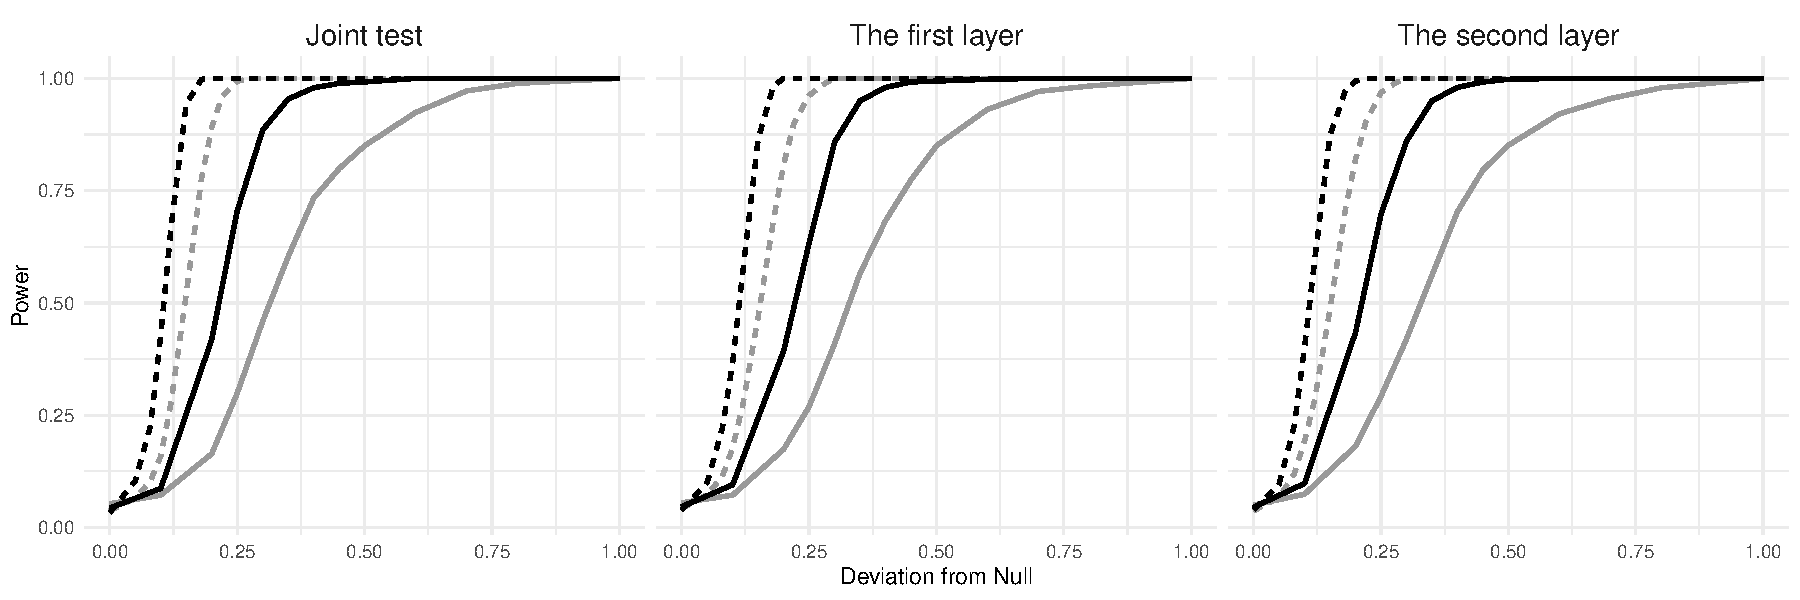
\includegraphics[width=\linewidth]{Exch.pdf}
%		\caption{Null: exchangeable covariance}
%		\label{fig:sub1}
%	\end{subfigure}%
%	\vskip 0.2\baselineskip
%	\begin{subfigure}{\textwidth}
%		\centering
%		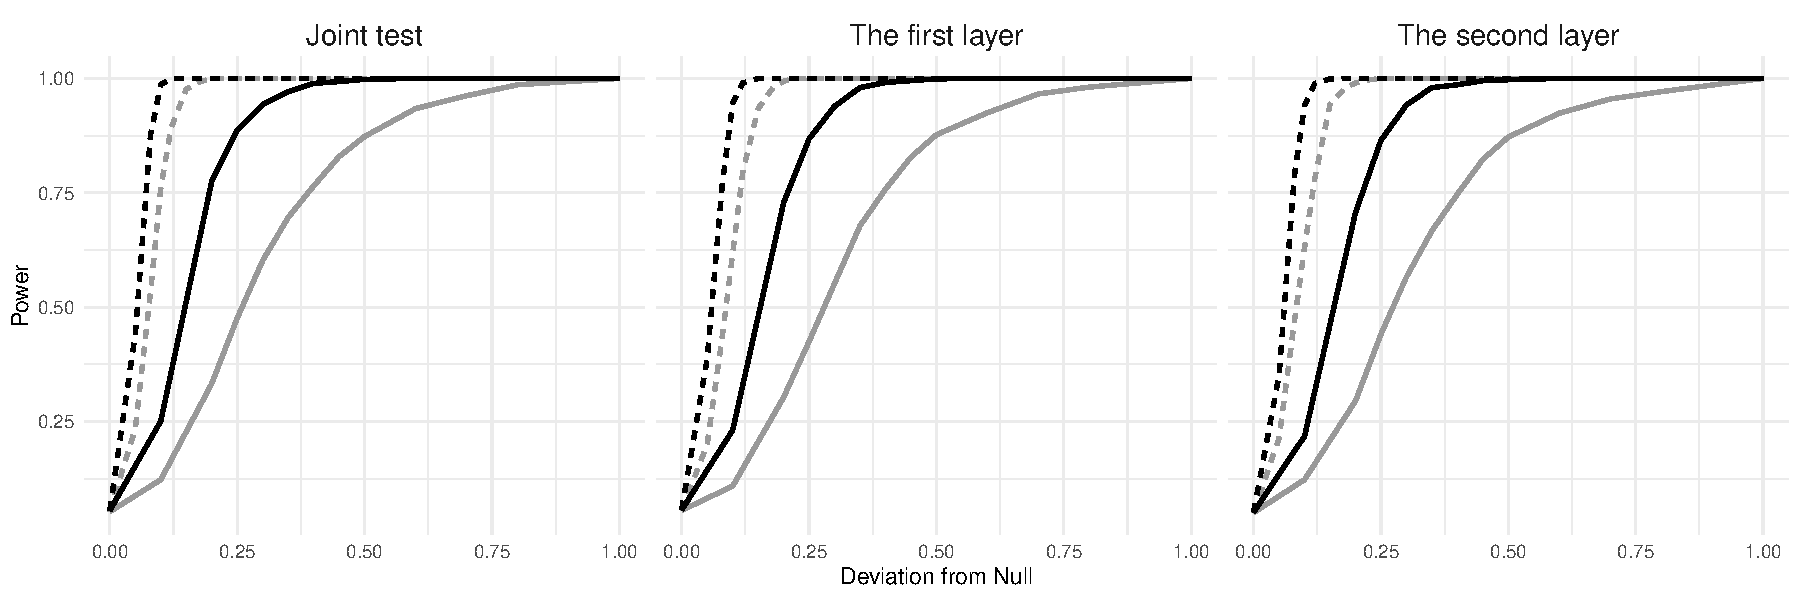
\includegraphics[width=\linewidth]{Indep.pdf}
%		\caption{Null: independent covariance}
%		\label{fig:sub2}
%	\end{subfigure}
%	\caption{Power curves (type \uppercase\expandafter{\romannumeral1} error $\alpha=0.05$) for individual and joint tests of covariances, under deviation from the null. Shown are:  $m_i \sim \text{Unif}[3,6]$ (solid line) and $m_i \sim \text{Unif}[8, 12]$ (dashed line), for $n=100$ (gray) and $n=200$ (black).}
%	\label{power}
%\end{figure}


\section{Data application}\label{sec:application}


Wearable devices such as accelerometers provide objective and detailed measurements of physical activity and enable researchers to study how physical activity changes with age, personal characteristics, and health status. In an earlier study based on cross-sectional data, \cite{Xiao2015} analyzed the systematic and random circadian rhythms of physical activity as functions of time of day and age; see also \cite{Goldsmith2015}.


In this analysis, our objective is to quantify the circadian rhythm of physical activity over multiple days and how they relate to age, sex and body mass index (BMI) and provide associated inference. Data were collected from the National Health and Nutrition Examination Survey (NHANES), a large cohort study conducted in two-year waves by the US Centers for Disease Control and Prevention (CDC) to assess the health and nutritional status of US population. We focus on the NHANES 2011-2012 and 2013-2014 data, where each study participant was asked to wear the wrist-worn device all the time for seven consecutive days. The physical activity data were collected and summarized in minute-level Monitor-Independent Movement Summary (MIMS) units, a physical activity intensity unit optimized to capture normal human motion \citep{John2019}. For each day of the study participant, our initial data are MIMS measured at $1440$ minutes from midnight to midnight. For simplicity, the data are summarized by taking the half-hourly average, resulting in $48$ observations that gives the daily activity profile as a function of the day's hour. We include sex (denoted by $\text{sex}_i$), age ($\text{age}_i$), and BMI ($\text{BMI}_{i}$) as the covariates in this analysis.


The final dataset consists of $513$ study participants ($208$ men and $305$ women) with an average age of $57$ years and an average BMI value of 28. For each study participant, we further subset the days with at least $95\%$ estimated wear time, leading to a total of $3187$ days of wear with an average of $6.21$ days of wear per study participant. For subject $i$ at day $j$, the average MIMS at hour $s$ of a day is our longitudinal functional outcome, denoted by $y_{ij}(s)$. 

We specify the mean function as $\mu_{ij}(s) = \beta_0(s) + \text{sex}_i\beta_{\text{sex}}(s) + \text{age}_{i}\beta_{\text{age}}(s) + \text{BMI}_{i}\beta_{\text{BMI}}(s)$. The variable $\text{sex}_i$ is $0$ for males and $1$ for females. Both age and BMI are centered so that $\beta_0(s)$ is the population mean MIMS corresponding to males of age $57$ and with BMI of $28$. The longitudinal covariate $T_{ij}$ is the day of wear. Considering the coefficient function can be thought of as on a circle where the end points of it should actually be equivalent(hour of day), the mean estimation is conducted using cyclic P-splines. To investigate the longitudinal correlation structure of the data,  we first estimate the marginal covariance function, which is estimated via the  {\it fpca.face} R function using cubic B-spline basis functions with $10$ knots. Using the procedure described in Section~\ref{sec:Modelestimation}, we identify that seven eigenfunctions explain $90\%$ of the marginal variance. Using these seven eigenfunctions, we conduct a joint test for the null hypothesis that all longitudinal covariances $G_{k0}(\cdot,\cdot)$ can be induced by an exchangeable covariance between daily profiels within each subject. The $p$-values are $0.042$, $0.259$, $0.039$, $0.500$, $0.454$, $0.204$ and $0.593$, respectively. Thus, with the Bonferroni correction, we do not reject the null hypothesis at the 0.05 level. Thus, for model fit, we use exchangeable covariance structure for all longitudinal covariances.


The estimated coefficient functions are displayed in Figure~\ref{fig:NHANES_beta}, along with the $95\%$ pointwise confidence bands. The top left panel in Figure~\ref{fig:NHANES_beta} displays the estimated mean activity profile $\beta_0(s)$ for males with age $57$ and BMI $28$. The shape is consistent with that of published average activity plots over the course of the day. On average, individuals are less active during night. Then, their activities  increase sharply between 5AM and 11AM, sustain between 11AM and 7PM, and decrease rapidly after 7PM. The top right panel indicates that females in this age group (50 to 70) have significantly more activities than males throughout most of the day except for midnight. The bottom left panel displays the estimated coefficient function for age, indicating a loss of activity for older individuals from afternoon to 1AM. There is no substantial age effect in activity in the morning  while the most considerable age effect happens in the early night. These findings are consistent with common sense that older individuals sleep early at night and wake up early in the morning, while younger individuals are more energetic at night. The bottom right panel indicates that activity patterns tend to decrease with increasing BMI, especially in the daytime. 

%\begin{figure}[!h]
%	\centering
%	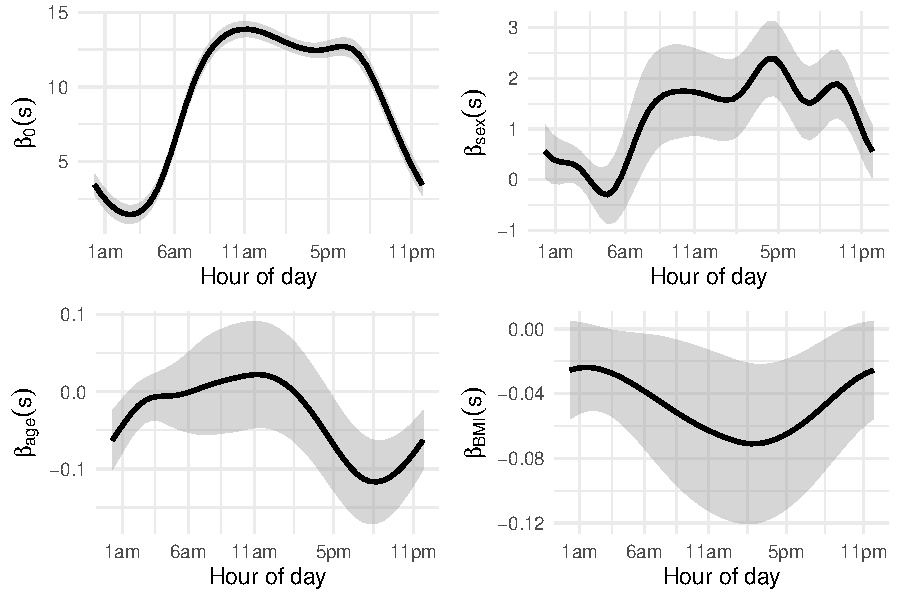
\includegraphics[width=\linewidth]{NHANES_exch48_cp.pdf}
%	\caption{ Estimated coefficient functions for the NHANES dataset along with pointwise $95\%$ confidence bands under exchangeable longitudinal covariance structure.} 
%	\label{fig:NHANES_beta}
%\end{figure}


Figure \ref{fig:NHANES_activity} displays the estimated mean activity profiles for females and males, with different age and BMI combinations. From the top panels, we see that for a given BMI value, there is a pronounced decrease in activity as a function of age, both for females and males. Moreover, younger individuals have on average two activity peaks, while older individuals tend to lose the second activity peak. It indicates that the change of physical activity patterns with age is due to less activity in the afternoon and at nigh. The bottom panels indicate that the average activity profile decreases with increasing BMI. The negative effect of age only works after noon while individuals with larger BMI have less activity during all daytime. Moreover, the effect of two units on the BMI scale is roughly equivalent to two years of age in terms of overall activity loss. 

%\begin{figure}[!h]
%	\centering
%	\begin{subfigure}{\textwidth}
%		\centering
%		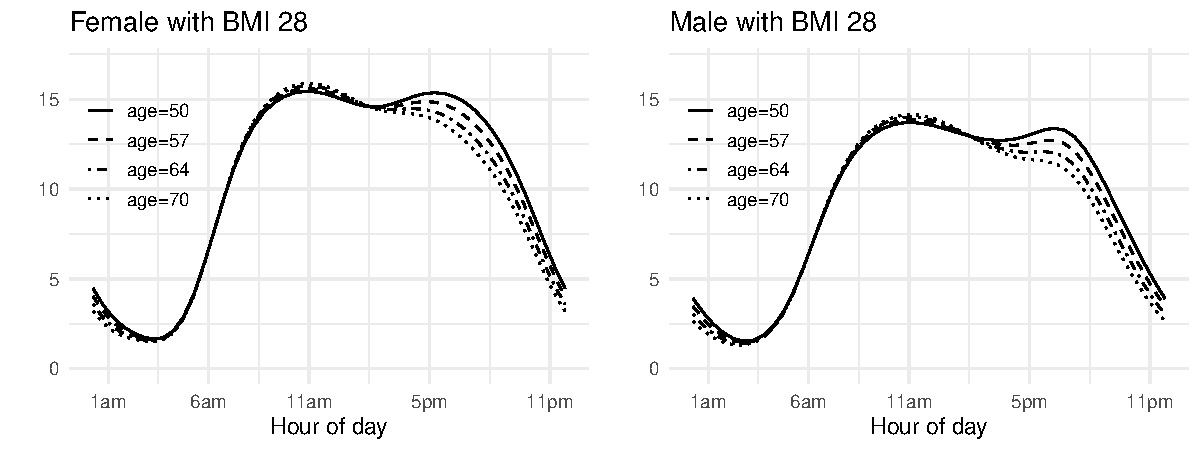
\includegraphics[width=\linewidth]{NHANES_age.pdf}
%	\end{subfigure}%
%	\vskip\baselineskip
%	\begin{subfigure}{\textwidth}
%		\centering
%		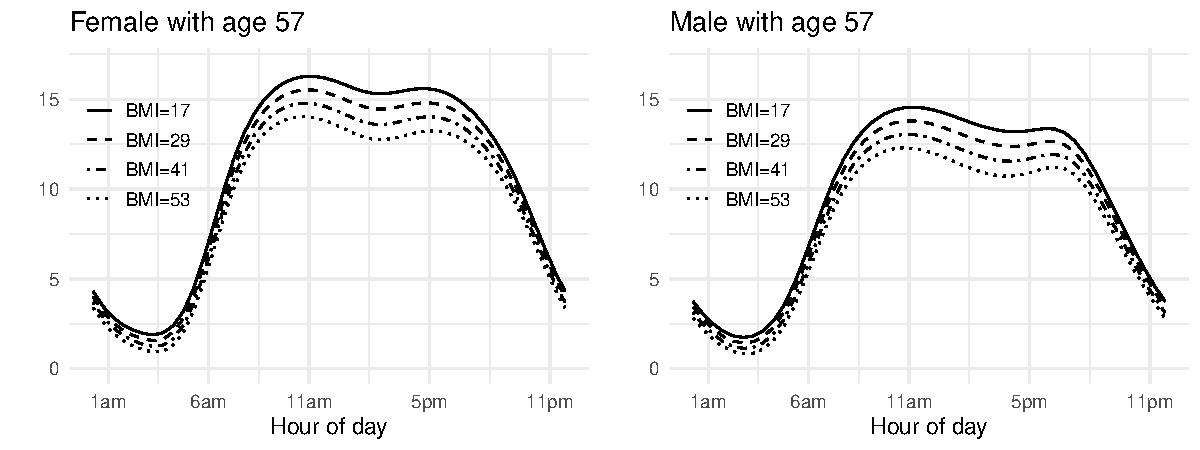
\includegraphics[width=\linewidth]{NHANES_BMI.pdf}
%	\end{subfigure}
%	\caption{ Top panels: estimated mean activity profiles of females and males with BMI $28$  at four different ages; bottom panels: estimated mean activity profiles of
%		females and males with age $57$ and with four different BMI values.}
%	\label{fig:NHANES_activity}
%\end{figure}




\section{Discussion}\label{sec:conclusions}
We introduced an inferential framework for estimating  fixed effects functions for longitudinal functional data with complex correlation structures. Methods are natural extensions of standard longitudinal data methods with scalar observations and use the flexible marginal decomposition model framework in \cite{Park2015}. 

Simulation studies indicate that the estimation procedure works remarkably well even when the longitudinal correlations are misspecified. However, the confidence bands obtained under misspecified correlation models may  have smaller than nominal coverage  or are wider than  necessary. Our results indicate that using unspecified correlation matrices is the safer approach when it is computationally feasible. More work will be necessary to improve the computational feasibility of these methods for larger sample sizes in terms of the number of study participants, visits, and observations per curve.

We also introduced a testing framework for longitudinal correlations for longitudinal functional data, which extended the testing method in \cite{Chen2019}. The proposed tests provide insight into what correlation structures are appropriate and may help reduce the computational cost  when a simpler longitudinal correlation is chosen.

The computer code to demonstrate the proposed method and a RMD file with details can be obtained from \url{https://github.com/rli20ST758/FILF} .

%%% Acknowledgements (if any)
%%% ------------------------------------------
%\section*{Acknowledgements}
%We want to thank\ldots


%%% References if bibTeX is used
%%%
%%% Please, do not specify any \bibliographystyle{} command!
%%%
%%% It is already specified in the smj.cls and its
%%% second specification here causes error.
%%% ------------------------------------------------------------
\bibliography{smj-template}



\end{document}
